
\usetikzlibrary{arrows.meta, positioning}

\begin{figure*}

    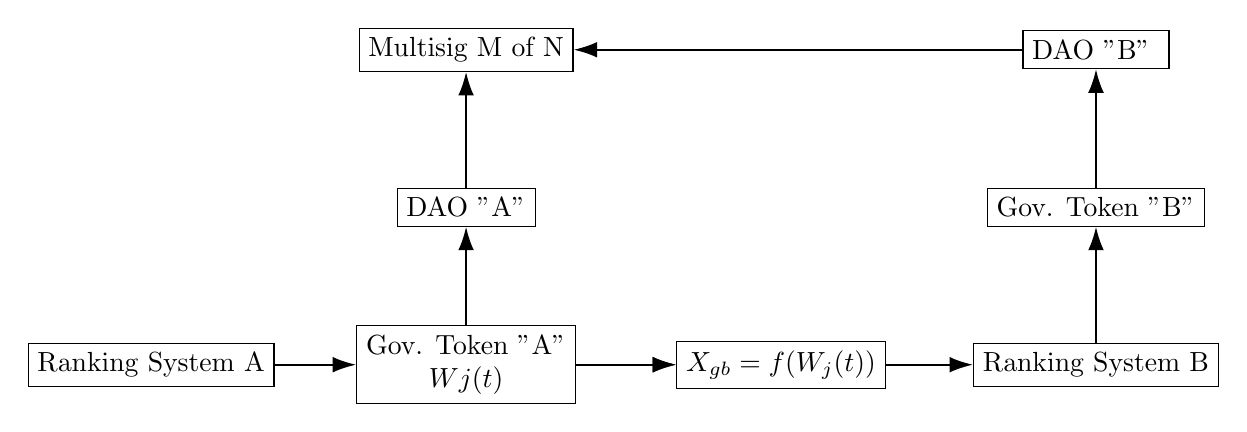
\begin{tikzpicture}[
        node distance=2cm,
        every node/.style={draw, align=center},
        arrow/.style={-{Latex[length=3mm, width=2mm]}, thick}
        ]


        % Single block for the game

        % Nodes
        \node (Competence_A) {Ranking System A};
        \node[right of=Competence_A, , xshift=2cm]  (A_token) {Gov. Token "A" \\ $Wj(t)$};
        \node[above of=A_token]  (DAO_origin) { DAO "A"};
        \node[above of=DAO_origin] (Multisig) {Multisig M of N};
        \node[right of=A_token, xshift=2cm] (exchanger) {$X_{gb} = f(W_j(t))$};
        \node[right of=exchanger, xshift=2cm] (Competence_B) {Ranking System B};
        \node[above of=Competence_B]  (B_token) {Gov. Token "B"};
        \node[above of=B_token]  (DAO_B) { DAO "B" };

        \draw [arrow] (Competence_A) -- (A_token);
        \draw [arrow] (A_token) -- (DAO_origin);
        \draw [arrow] (DAO_origin) -- (Multisig);
        \draw [arrow] (A_token) -- (exchanger);
        \draw [arrow] (A_token) -- (exchanger);
        \draw [arrow] (exchanger) -- (Competence_B);
        \draw [arrow] (Competence_B) -- (B_token);
        \draw [arrow] (B_token) -- (DAO_B);
        \draw [arrow] (DAO_B) -- (Multisig);






    \end{tikzpicture}
    \caption{Diagram describing progressive decentralization via DAO composition. As initial group governing DAO "A" experiences inflation it may provision next organization "B" to focus on specific aspects of arbitrary protocol, and maintain any asset security by moving them further on to the governance  chain. If such assets are assigned to multisig, original DAO value is preserved, therefore allowing organization to grow both horizontally and vertically.  }
    \label{fig:dao-composition}
\end{figure*}